\section{Differences in Treetank}\label{sec::differences}
\subsection{Introduction}
This chapter describes the need for two kinds of difference algorithms and how they are implemented in Treetank, which is used as backend to demonstrate our approach to determine and visualize changes in tree-structures. First, Treetank is depicted. Then it is described why 

\subsection{Storage}
Treetank, as meantioned before, is an effective and efficient secure storage system tailored to temporal tree data. Currently it supports the import of XML documents which is called \emph{shredding}. To process stored data the W3C recommendations XPath 2.0, XQuery 1.0 and XSLT 2.0\footnote{parts of the XPath 2.0 recommendation have been implemented, alternatively the Saxon XPath 2.0 binding can be used which also offers the XQuery 1.0 and XSLT 2.0 support}, as well as a cursor like Java-API is supported. The architecture is based on three exchangeable horizontal aligned layers. What follows is a brief description of each layer in a top-down approach:

\begin{description}
\item[Transaction] Transactions are divided into \texttt{read}- and \texttt{write}-transactions. Read-Transactions are able to read stored nodes through a cursor-like API. Write-Transactions extend the functionality of Read-Transactions. They provide methods to modify data and commit the changes to store a new revision. Changes are atomar and saved in a Pending Update List (PUL)/transaction log which literally means they are either commited at a whole or aborted which triggers a rollback. Therefore in the latter case all modifications done within this transaction after the last commit aren't persisted and lost. Every transaction owns a unique transaction ID as well as a timestamp which denotes the last commit-time of the transaction.
\item[Node] The node layer is responsible for providing different node kinds. Currently \texttt{comment} and \texttt{processing instruction} nodes are not supported due to the  research prototype implementation which is sufficient in almost all cases. Note that adding these two node types wouldn't be a big deal. The node- and transaction-layer are responsible for the storage encoding. Since updates have to be performant for now the encoding is implemented as storing all neighbour structural nodes \footnote{all node kinds except attribute and namespace nodes} for every node. This results in a local \texttt{key/parentKey/firstChildKey/[left|right]SiblingKey} encoding further illustrated in figure \ref{fig:encoding}. Inserting a structural node either involves calling \texttt{insertAsFirstChild()} or \texttt{insertAsRightSibling()} on a write transaction. The first case requires to set

\begin{itemize}
\item the parent key to the current key located at the current transaction cursor position (before the insert)
\item a special \texttt{NULL\_NODE\_KEY} to mark the nonexistence of any left sibling
\item the former first child as the right sibling
\end{itemize}

The latter case requires to set

\begin{itemize}
\item the parent key to the current parent key
\item the left sibling key to the current node key
\item the right sibling key to the current right sibling key
\end{itemize}

\begin{figure}[tb]
\centering
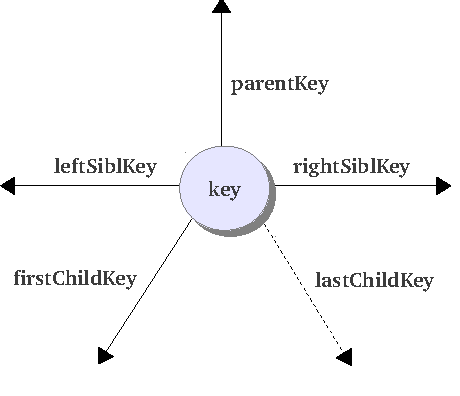
\includegraphics[width=0.45\textwidth]{figures/encoding}
\caption{Treetank encoding} 
\label{fig:encoding}
\end{figure}

Besides fixed length data, as the pointers to neighbour nodes, variable content might be stored in the node itself. For instance a hash which is used for ensuring integrity of the nodes' subtree and build through the references between the nodes is stored. In our context these hashes set the stage for efficient generation of diffs based on a simple comparsion of the hash values which is described later on in this chapter.

\item[Page] The page-layer is motivated by ZFS \todo{REFERENZ}. It takes care of persisting nodes and is designed for the efficient storage of versioned tree-structures. Based on the copy-on-write (COW) principle no data is lost. Once a write transaction commits changes new NodePages are persisted, which include all modified nodes including affected neighbour/parent/child nodes. The architecture is illustrated in figure \todo{REFERENZ}.
\end{description}

This architecture supports \emph{Snapshot-Isolation} through \emph{MVCC} (Multiversion Concurrency Control).

\subsection{Preprocessing}
Preprocessing of raw data is one of the major tasks. Databases which haven't evolved through the revisioned storage in Treetank have to be imported. To take full advantage of the decreased storage costs regarding revisioned in Treetank first of all differences between several full dumps have to be computed. Note that it is very common to simply dump full revisions of time-varying data and to collect data which evolves through snapshots of the full data.

For the simple reason that Treetank currently offers a convenient XML node layer, we concentrate our effort on importing XML data. As most XML-documents don't incorporate unique node IDs the FMSE algorithm described in the last chapter has been implemented. The reason for chosing FMSE is simply that it has been implemented to build a delta between XML-documents at least three times. To support the actual FMSE implementation Treetank has been enhanced in several ways:

\begin{itemize}
\item \texttt{LevelOrderAxis} which incorporates attribute- and namespace-nodes if desired
\item \texttt{copy-operation} to copy subtrees of other \emph{database/resource}-tuples
\item \texttt{move-operation} to move subtrees in the currently opened \emph{resource}
\item visitor pattern support for nodes/transactions
\end{itemize}

The \texttt{LevelOrderAxis} is described in algorithm \ref{levelOrderAxis}. Just like other axis in Treetank it is based on the \texttt{Iterator/Iterable} Java interfaces to support the \texttt{foreach}-loop and iteration. The check if \texttt{getNext()} is true was added to all axis such that \texttt{hasNext()} is idempotent. It simply checks a flag which is set in \texttt{resetToLastKey()} which is also invoked to make sure the transaction points to the node after the last \texttt{hasNext()}. \emph{mFirstChilds} is a queue to remember all first childs from every right sibling for a subsequent new depth (depth + 1). \texttt{processElement()} is invoked to add non structural nodes, that is \texttt{attributes} and \texttt{namespaces} to the queue. After initialisation the queue is empty and \emph{mNextKey} is initialized to either the current key (if self is included), the right sibling node key if there is one or the first child node key. The NULL\_NODE\_KEY is a special node key to denote that the traversal is done.

\begin{algorithm}[Hhtbp]
%\SetAlgoLined
\SetKwInOut{Input}{input}\SetKwInOut{Output}{output}
\Input{instance variables (denoted by a trailing "m")}
\Output{node key of next node}
\BlankLine
\If{getNext()}{
  return true\;
}
  resetToLastKey()\;

  \tcp{Fail if there is no node anymore.}
  \If{mNextKey $\leftarrow$ NULL\_NODE\_KEY}{
    resetToStartKey()\;
    return false\;
  }

  \tcp{First move to next key.}
  mRtx.moveTo(mNextKey)\;

  \tcp{Follow right sibling if there is one.}
  \If{mRtx.getStructuralNode().hasRightSibling()}{
    processElement()\;
    \tcp{Add first child to queue.}
    \If{mRtx.getStructuralNode().hasFirstChild()}{
      mFirstChilds.add(mRtx.getStructuralNode().getFirstChildKey())\;
    }
    mNextKey $\leftarrow$ mRtx.getStructuralNode().getRightSiblingKey()\;
    return true\;
  }

  \tcp{Iterate over non structural nodes (attributes/namespaces).} 
  \If{mInclude equals EInclude.NONSTRUCTURAL}{
    processElement()\;
  }
  \tcp{Add first child to queue.}
  \If{mRtx.getStructuralNode().hasFirstChild()}{
    mFirstChilds.add(mRtx.getStructuralNode().getFirstChildKey())\;
  }

  \tcp{Then follow first child on stack.}
  \If{!mFirstChildKeyList.isEmpty()}{
    mNextKey $\leftarrow$ mFirstChilds.remove(0)\;
    return true\;
  }

  \tcp{Then follow first child if there is one.}
  \If{mRtx.getStructuralNode().hasFirstChild()}{
    mNextKey $\leftarrow$ mRtx.getStructuralNode().getFirstChildKey()\;
    return true\;
  }

  \tcp{Then end.}
  mNextKey $\leftarrow$ NULL\_NODE\_KEY\;
  return true\;
\caption{LevelOrderAxis (hasNext())}\label{levelOrderAxis}
\end{algorithm}

The \texttt{copy}-operation adds the capability to add whole subtrees of another \emph{database/resource} tuple to the currently opened \emph{resource}. Therefore and to support
many different kinds of operations depending on different node kinds the visitor pattern is used.

\begin{algorithm}[Hhtbp]
\SetKwInOut{Input}{input}\SetKwInOut{Output}{output}
\Input{instance variables (denoted by a trailing "m"), TextNode pNode}
\Output{void (none)}
\BlankLine
mRtx.moveTo(paramNode.getNodeKey())\;
mInsert.insertNode(mWtx, mRtx)\;

\If{!mFirst $and$ mRtx.getStructuralNode().hasRightSibling()}{
  mRtx.moveToRightSibling()\;
  mInsert $\leftarrow$ EInsert.ASRIGHTSIBLING\;
  mRtx.getNode().acceptVisitor(this)\;
}\ElseIf{!mFirst}{
  insertNextNode();
}
\caption{visitTextNode(TextNode pNode))}\label{visitTextNode}
\end{algorithm}

\begin{algorithm}[Hhtbp]
\SetKwInOut{Input}{input}\SetKwInOut{Output}{output}
\Input{instance variables (denoted by a trailing "m"), ElementNode pNode}
\Output{void (none)}
\BlankLine
mRtx.moveTo(pNode.getNodeKey())\;
mInsert.insertNode(mWtx, mRtx)\;
\If{pNode.getNamespaceCount() $>$ 0}{
  mInsert $\leftarrow$ EInsert.ASNONSTRUCTURAL\;
  \For{int i = 0; i $<$ paramNode.getNamespaceCount(); i++}{
    mRtx.moveToNamespace(i)\;
    mInsert.insertNode(mWtx, mRtx)\;
    mRtx.moveToParent()\;
  }
}

\If{paramNode.getAttributeCount() $>$ 0}{
  mInsert $\leftarrow$ EInsert.ASNONSTRUCTURAL\;
  \For{int i = 0; i $<$ paramNode.getAttributeCount(); i++}{
    mRtx.moveToAttribute(i)\;
    mInsert.insertNode(mWtx, mRtx)\;
    mRtx.moveToParent()\;
  }
}

\If{pNode.hasFirstChild()}{
  mFirst $\leftarrow$ false\;
  mInsert $\leftarrow$ EInsert.ASFIRSTCHILD\;
  mRtx.moveToFirstChild()\;
  mDepth+=1\;
  mRtx.getNode().acceptVisitor(this)\;
}\ElseIf{!mFirst $and$ paramNode.hasRightSibling()}{
  mInsert $\leftarrow$ EInsert.ASRIGHTSIBLING\;
  mRtx.moveToRightSibling()\;
  mRtx.getNode().acceptVisitor(this)\;
}\ElseIf{!mFirst}{
  insertNextNode()\;
}
\caption{visitElementNode(ElementNode pNode))}\label{visitElementNode}
\end{algorithm}

\begin{algorithm}[Hhtbp]
\SetKwInOut{Input}{input}\SetKwInOut{Output}{output}
\Input{instance variables (denoted by a trailing "m")}
\Output{void (none)}
\BlankLine
\While{!mRtx.getStructuralNode().hasRightSibling() and mDepth $>$ 0}{
  mRtx.moveToParent()\;
  mWtx.moveToParent()\;
  mDepth-=1\;
}

\If{Depth $>$ 0}{
  mInsert $\leftarrow$ EInsert.ASRIGHTSIBLING\;
  \If{mRtx.getStructuralNode().hasRightSibling()}{
    mRtx.moveToRightSibling()\;
    mRtx.getNode().acceptVisitor(this)\;
  }
}
\caption{insertNextNode()}\label{insertNextNode}
\end{algorithm}

To demonstrate the feasability of our analysis system with real world data, a Wikipedia dump as well as a   has been used.

\subsubsection{Wikipedia} is dumped as a very big XML file. "'The XML itself contains complete, raw text of every revision"' \todo{REFERENZ} and thus is a full dump instead of an incremental or differential dump which could be used in conjunction with the latest full dump. Moreover WikiText, which is a proprietary markup format is stored as plain text. As a consequence differences between two revisions of an article couldn't be found with a state of the art native XML revisioning database system. 

Furthermore due to the fact that XPath 2.0 should be usable without requiring an XPath Full Text 1.0 implementation and our overall goal is to analyse the temporal nature of the stored data, WikiText markup has to be converted into semistructured XML fragments. To accomplish this the Wiki2XML parser from the MODIS team \todo{REFERENZ} is used.

Next the Wikipedia dump isn't sorted. Neither articles are sorted by date nor revisions inside articles are. Thus for the subsequent revisioned import the revisions have to be sorted with their associated article metadata (page id, author...). Since we have to deal with large amounts of data external sorting algorithms had to be considered. Instead of implementing an own approach Hadoop seemed to be a natural choice. It's \emph{MapReduce} framework is a "programming model and software framework for writing applications that rapidly process vast amounts of data in parallel on large clusters of compute nodes". The overall process of the programming model is divided into two functions.

\begin{enumerate}
\item \texttt{Map} is a function that has the task of splitting the problem into subproblems which can be distributed over worker nodes in a cluster. Logically it is a function of the form $Map(k1,v1) \rightarrow list(k2,v2)$ where $k1$ and $v1$ is an input $key$ and $value$ and the output from the function is a list of $key/value$ pairs ($list(k2, v2)$). After that the MapReduce framework groups the values according to the keys.
\item \texttt{Reduce} is a function of the form: $Reduce(k2, list (v2)) \rightarrow list(v3)$. It receives a $key$ and a list of grouped $values$ and returns performs any computation which might be feasable and returns another list of $values$.
\end{enumerate}

Using the map-function means input data has to be split into records. Most MapReduce frameworks rely on some mechanism to do this. In Hadoop the \texttt{InputStream} in conjunction with a \texttt{RecordReader} takes this responsibility. The following steps describe the implementation of sorting Wikipedia by Hadoop.

\begin{enumerate}
\item \texttt{XMLInputStream} in conjunction with an \texttt{XMLRecordReader} splits records on \emph{page-elements}. The \textbf{timestamp} of each revision is used for the key, the whole subtree of each \emph{page-element} is saved as the value for the map input. The algorithm is straight forward. A \texttt{SAX-Parser} is used to determine starting and ending of each record. The algorithm is outlined in \ref{splitRecs}


\begin{algorithm}[Hhtbp]
%\SetAlgoLined
\KwData{preprocessed Wikipedia XML dump}
\KwResult{splitted records; $key \leftarrow timestamp$ of latest revision in $page$\; $value \leftarrow page$ with all revisions}
$parser \leftarrow StAX-Parser$ at the beginning of the XML document\;
$timestamp \leftarrow dummydate$\;
$isTimestampNode \leftarrow false$\;
$list \leftarrow empty$\;
\While{parser.hasNext()}{
$node \leftarrow parser.next()$\;
\If{$node$.isStartElement() {\bf{and}} $node \leftarrow isPage$}{
$list$.add($node$)\;
}\ElseIf{$node$.isEndElement() {\bf{and}} $node \leftarrow isPage$}{
emit $timestamp/list$ tuple\;
}\ElseIf{$node$.isStartElement() {\bf{and}} $node \leftarrow isTimestamp$}{
$isTimestampNode \leftarrow true$\;
}

\If{$isTimestampNode \leftarrow true$}{
$isTimestampNode \leftarrow false$\;
$timestamp \leftarrow node$\;
}
}
\caption{SplitRecords}\label{splitRecs}
\end{algorithm}

Note that the actual implementation uses record identifier such that it can be used with every other XML file and other split nodes as well.

\item \texttt{XMLMap} is responsible for breaking up each page into revision chunks and once more store the timestamp of each revision as the key whereas the value this time consists of the metadata of each page and exactly one revision.
\item \texttt{XMLReduce} finally merges consecutive revisions with the same \emph{page-id} and \textbf{timestamp} by means of Saxon, an XSLT-processor among other things. The XSLT stylesheet used is pretty small yet maybe not straight forward. It is shown in listing \ref{combine}.

\begin{lstlisting}[caption=XSLT stylesheet to combine consecutive pages/revisions]
<xsl:stylesheet version="2.0" 
  xmlns:xsl="http://www.w3.org/1999/XSL/Transform" 
  xmlns:xs="http://www.w3.org/2001/XMLSchema"
  exclude-result-prefixes="xs">

  <xsl:output method="xml" indent="no" 
    omit-xml-declaration="yes" />
  <xsl:strip-space elements="*" />

  <xsl:template match="/">
    <xsl:copy>
      <xsl:for-each-group 
        select="descendant-or-self::page" 
        group-by="concat(id, revision/timestamp)">
        <page>
          <xsl:copy-of select="* except revision" />
	  <xsl:for-each-group 
            select="current-group()/revision"
	    group-by="xs:dateTime(timestamp)">
	    <xsl:apply-templates 
              select="current-group()" />
	  </xsl:for-each-group>
        </page>
      </xsl:for-each-group>
    </xsl:copy>
  </xsl:template>

  <xsl:template match="revision">
    <xsl:copy-of select="." />
  </xsl:template>
</xsl:stylesheet>
\end{lstlisting}
\label{combine}
\end{enumerate}

% import of wikipedia
Once it is sorted with MapReduce it has to be imported into Treetank. Therefor an Import class is written which implements the \texttt{IImport}-Interface. This class makes heavy use of the \texttt{XMLUpdateShredder} which is written to shred only incremental changes between the latest stored revision in Treetank and a new XML file or List of \texttt{XMLEvent}s. It is saved for further explanation in this chapter later on. The Import of Wikipedia allows the usage of a time slot (hourly, daily, monthly, yearly) which is used for the revisioning.

% import of network data

\todo{import wikipedia}
\todo{import network data}
\todo{describe algorithm}
\subsection{Data Mining}
Wikipedia defines Data Mining as:

\begin{quote}
Data mining is the process of extracting patterns from data. Data mining is becoming an increasingly important tool to transform this data into information. It is commonly used in a wide range of profiling practices, such as marketing, surveillance, fraud detection and scientific discovery.
\end{quote}

See that interesting patterns in respect to temporal data should be revealed our main concern is to discover changes. Therefore Treetank has to support different diff-calculations between two revisions.

One of our goals is the efficiency of our approach since it should be usable within interactive visualizations. Meantioned briefly in the storage section hashes of the nodes can be used to skip traversal of subtrees. Whenever equal hashes are determined the two transactions which compute the diff can move to the right sibling. To encapsulate the main algorithm with the movement of the transactions from the actual diff calculation the strategy design pattern has been used. Interested observers are furthermore notified of the diff between two nodes through the implementation of a special interface method and registration. Currently two kinds of diffs can be computed.

\subsubsection{Structural Diff} calculates changes without comparing attribute and namespace nodes. This implies that whenever the overall structure is crucial this algorithm should be choosed \todo{ALGORITHM}.
\subsubsection{Full Diff} takes structural nodes as well as attribute and namespace nodes into account \todo{ALGORITHM}.
\todo{Diff construction}
\todo{text clustering}
\subsection{GUI}
The GUI is designed to be easily extendable. It currently offers the ability to view and interact with the stored Treetank data in many ways. Incorporated are several different views. A few of them are developed to be usable in the context of \emph{Visual Analytics}. Besides providing the basis for analysis the views are synchronized meaning that every change a view does to the underlying data or just the selection of nodes reflects itself in all other views, too. The implementation of this mechanisms relies on the well known \emph{observer pattern}. Other software design patterns are extensively used all along, for example the \emph{strategy pattern} for menu items, the \emph{iterator pattern} to encapsulate the models in the \textbf{SunburstView} and so on.
\todo{brief description of non temporal views}
\subsection{Visualizations}
Visualizations are one of the major contributions in this thesis. A few of them concentrate on gaining further insight into one revision. 

\begin{itemize}
\item
First a \textbf{TreeView} displays nodes in a tree structure like shown in \todo{FIGURE}. Nodes can be expanded to show all child nodes which are inside the current viewport or collapsed to hide children. Therefore a JTree is used which has been extended to mark the subtree of a selected node with a background color. The \texttt{TreeCellRenderer} renders nodes according to their node type and a \texttt{TreeModel} interacts with the storage. 

\item
The \textbf{TextView} shows simple serialized XML fragments and supports syntax highlighting. Moreover it just serializes the part of data which is currently viewable. Other data is serialized and appended to the text pane once a user drags the scroll pane. Implementation wise it is done through the usage of a \emph{StAX}-Parser which supports a pull based API. It provides two features. Since it is pull based the application (the GUI) can determine when and how much data is parsed. Furthermore it provides the parsed node kinds which are used to support syntax highlighting. The algorithm to implement a StAX-Parser for Treetank is outlined in \todo{REFERENZ}. 

\item
A \textbf{SunburstView} can be used to view the tree structure in a circular arrangement. It is a space filling approach even though unlike in TreeMaps the corners are left empty due to the radial representation. The descendant-count is mapped onto the extend of each segment meaning that nodes with more descendants are plotted with a greater extend. The formular is straight forward:

\begin{equation}
ext = \left\{ \begin{array}{cl}
parExt & \textrm{if }node\ is\ leaf\ node\\
parExt * descs / parDescs & \textrm{otherwise}\end{array}\right.
\end{equation}

%\begin{equation}
%currExt = parExt * descCount / parDescCount
%\end{equation}

The color of each segment is mapped to the number of child nodes or to the text size length for leaf nodes. Nodes are furthermore visualized through circles and bezier curves from the current node to the parent node highlight the hierarchical relationships. Through checkboxes the dots/circles and/or the arcs can be hidden. Moreover the size of the dots can be managed through a slider.

\end{itemize}

To guide analysts in gaining knowledge from the stored data besides automatic clustering and views which only concentrate on one revision a few interactive visualizations have been developed to compare different revisions. The first one, an extended SunburstView reveals changes between two revisions. The user can therefore choose between a few diff-algorithms which have been already described. Changes are revealed through the mapping of space to the extend of a Sunburst segment and the color. The first revision is plotted in the center of the screen. The changes from the old (first) revision to the new revision are plotted in a circular arrangement around the first revision supporting a TreeRing metapher. Users can choose to what dimension the changes are reflected in the extend of the Sunburst segment. The formula is as follows:

\begin{equation}
ext = \left\{ \begin{array}{cl}
(1-\alpha) * parExt * descs / parDescs & \textrm{if }descs\ or\ parDescs == 0\\
\alpha * parExt * diffs / parDiffs\\
+ (1-\alpha) * parExt * descs / parDescs & \textrm{otherwise}\end{array}\right.
\end{equation}

\todo{describe extended SunburstView}
\todo{describe extended node link diagram}

\subsection{Interaction}
The simple \emph{SunburstView} as well as the temporal views are highly interactive.

\subsubsection{Pruning}
Enabling pruning speeds up the initialization of the views. Several nodes can be skipped while querying the database in the model varying with the pruning approach.

\subsubsection{Modification}
The \emph{SunburstView} allows the modification of nodes. They can be inserted, renamed or deleted. Furthermore it allows movement of whole subtrees through a drag \& drop operation. 

\subsubsection{Normalizations}
The colors in the two SunburstViews indicate normalized values. Various normalizations can be choosen interactively to take different data sets into account.

\begin{description}
\item[linear]
\item[logarithmic]
\item[square root]
\end{description}

\subsubsection{Fisheye}
A fisheye transformation provides some kind of a magnifier to support the exploration of very small sunburst items with a small extend. The basic idea is that relevant information is presented in greater detail whereas other information is abstracted.

\subsubsection{Zooming/Panning}
Like the fisheye transformation zooming/panning allows to further investigate regions of interest. It is based on affine transformations.
